\begin{tcolorbox}[title=Stack and Queue definition,coltitle =black,fonttitle=\large\bfseries,colback=green!5!white,colframe=green!75!black]
	Stack and Queue are special uses of List in Python, with specific constraints:
	\begin{itemize}
		\item Stack: only add/remove element from one end (LIFO).
		\item Queue: Add at one end, remove from the other one (FIFO).
	\end{itemize}
	Queues and stacks share a common interface:
	\begin{itemize}
		\item push - adds an element. (For queues, this is also known as enqueue).
		\item pop - queries/removes an element. (For queues, this is also known as dequeue).
	\end{itemize}
\end{tcolorbox}

\subsection{Stack}
\subsubsection{Stack Visualization}
\begin{figure}[H]
	\centering 
	\begin{minipage}[b]{0.45\textwidth}
		\raggedright
		Stacks return elements in the reverse order in which they are stored; that is, the most recent element to be added is returned. We call this kind of data structure last-in-first-out (LIFO).
	\end{minipage}
	\hfill
	\begin{minipage}[c]{0.3\textwidth}
		\centering
		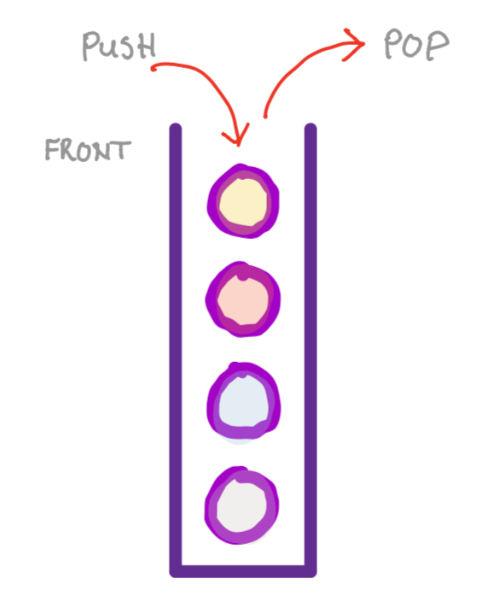
\includegraphics[width=\linewidth]{figures/stack-animation}
		\caption{Stack visualized}
	\end{minipage}
\end{figure}

\subsubsection{Push/Pop Visualization}
\begin{figure}[H]
		\centering
		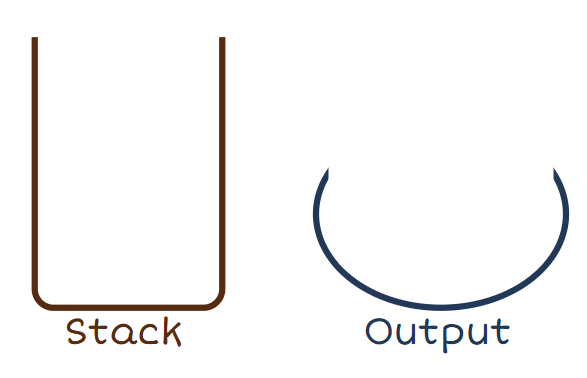
\includegraphics[width=0.45\textwidth]{figures/empty-stack}
		\caption{Create an Empty stack}
\end{figure}
\begin{figure}[H]
	\centering
	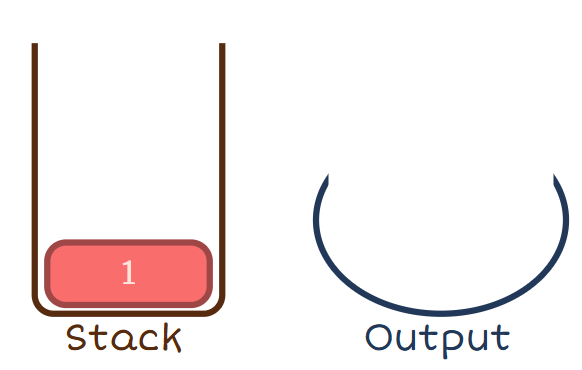
\includegraphics[width=0.45\textwidth]{figures/push-1}
	\caption{Push in the first element}
\end{figure}
\begin{figure}[H]
	\centering
	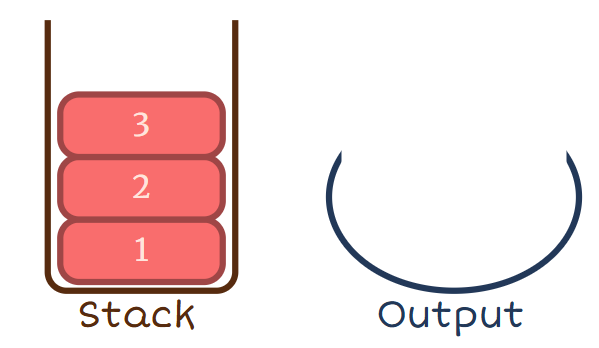
\includegraphics[width=0.45\textwidth]{figures/push-2-3}
	\caption{Push in the second and third element}
\end{figure}
\begin{figure}[H]
	\centering
	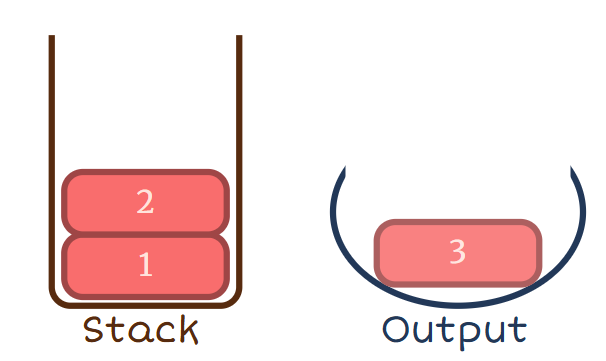
\includegraphics[width=0.45\textwidth]{figures/pop-3}
	\caption{Pop out the element at the top of the stack}
\end{figure}

\subsubsection{Coding}
\begin{lstlisting}[language=python, caption={Define Stack data structure class}]
	class MyStack:
		def _init_(self, capacity):
			self._capacity = capacity
			self._stack = []
			
		def push(self, value):
			if self.is_full():
				print('Do nothing!')
			else: 
				self._stack.append(value)
				
		def pop(self):
			if self.is_empty():
				print('Do nothing')
				return None
			else:
				return self._stack.pop()
			
		def print(self):
			print(self._stack)
			
		def is_full(self):
			return len(self._stack) == self._capacity
\end{lstlisting}

\begin{lstlisting}[language = python, caption={Push and Pop example}]
	stack1 = MyStack(5)
	stack1.push(12)
	stack1.push(8)
	stack1.push(21)
	stack1.push(33)
	stack1.push(34)
	stack1.push(35)
	stack1.print()
	
	//Output: Do nothing!
			  [12, 8, 21, 33, 34]	  
\end{lstlisting}

\subsection{Queue}
\subsubsection{Queue Visualization}
\begin{figure}[h]
	\centering 
	\begin{minipage}[b]{0.45\textwidth}
		\raggedright
		Queues return elements in the order in which they were stored. We call this kind of data structure first-in-first-out (FIFO).
	\end{minipage}
	\hfill
	\begin{minipage}[c]{0.3\textwidth}
		\centering
		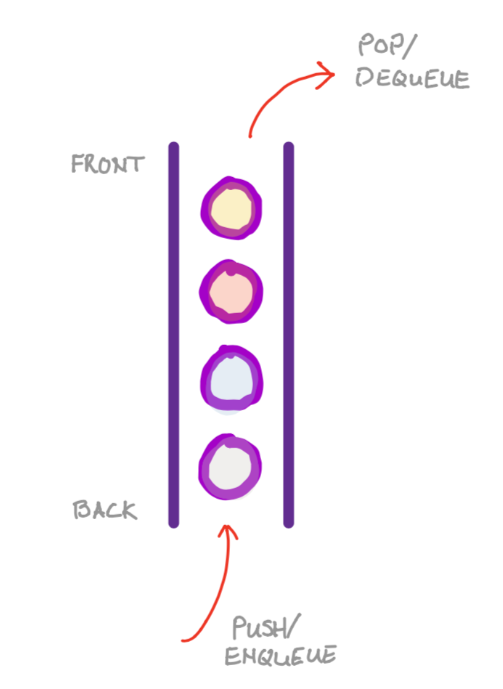
\includegraphics[width=\textwidth]{figures/queue-animation}
		\caption{Queue visualized}
	\end{minipage}
\end{figure}

\subsubsection{Queue/Dequeue Visualization}
\begin{figure}[H]
	\centering
	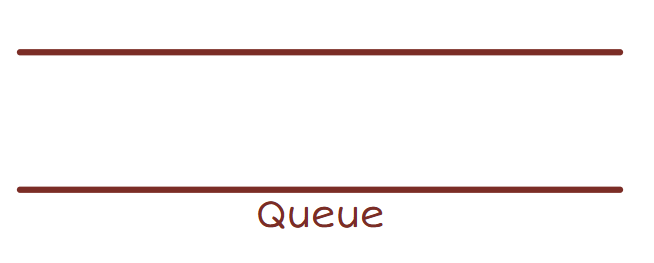
\includegraphics[width=0.45\textwidth]{figures/empty-queue}
	\caption{Create an Empty Queue}
\end{figure}
\begin{figure}[H]
	\centering
	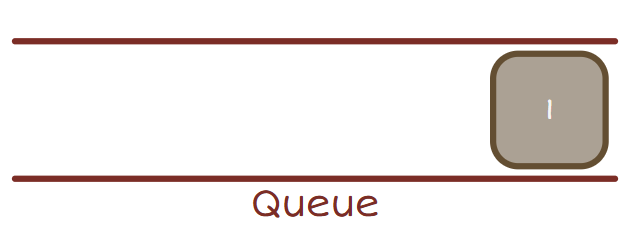
\includegraphics[width=0.45\textwidth]{figures/queue-1}
	\caption{Enqueue the first element}
\end{figure}
\begin{figure}[H]
	\centering
	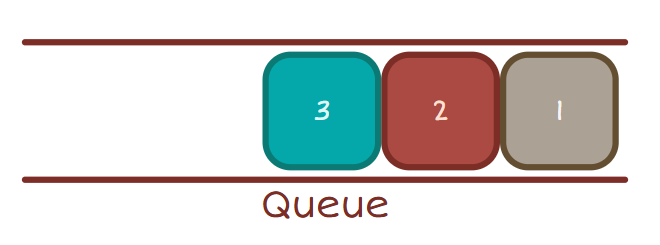
\includegraphics[width=0.45\textwidth]{figures/queue-2-3}
	\caption{Enqueue the second and third element}
\end{figure}
\begin{figure}[H]
	\centering
	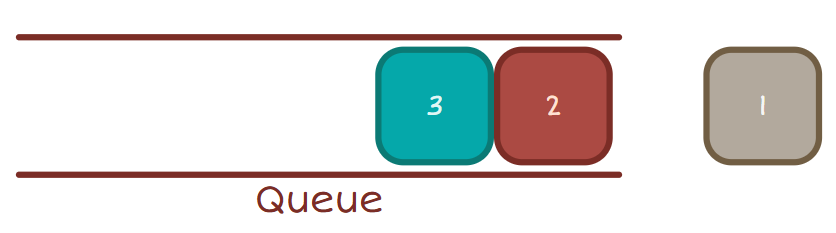
\includegraphics[width=0.45\textwidth]{figures/dequeue}
	\caption{Dequeue the element at the front of the queue}
\end{figure}

\subsubsection{Coding}
\begin{lstlisting}[language = python, caption={Define Queue data structure class}]
	class MyQueue:
		def _init_(self, capacity):
			self._capacity = capacity
			self._data = []
		
		def is_empty(self):
			return len(self._data) == 0
			
		def dequeue(self):
			if self.is_empty():
				print('Do nothing')
				return None	
			else: 
				return self._data.pop(0)
		
		def print(self):
			print(self._data)
\end{lstlisting}

\begin{lstlisting}[language = python, caption={Example}]
	queue = MyQueue(5)
	queue.print()
	
	queue.enqueue(9)
	queue.enqueue(5)
	queue.enqueue(2)
	queue.enqueue(1)
	queue.enqueue(0)
	queue.enqueue(6)
	
	//Output:
	Do nothing!
	[9, 5, 2, 1, 0]
\end{lstlisting}
